\documentclass[../main.tex]{subfiles}
\usepackage{fancyhdr}
\graphicspath{{../images/}}

\begin{document}
\pagestyle{fancy}
\lhead{Physics 472: Li Yang}
\chead{Homework 4}
\rhead{Junseo Shin}

\renewcommand\thefigure{\arabic{figure}} 
\paragraph*{Problem 1.} For a Fermi Gas in 3D we assume a sphere in $k$-space with radius $k_F$
and volume $\frac{4}{3} \pi k_F^2$. For each volume element we have 3D potential well with 
a plane wave solution $k^3 = \qt(\frac{2\pi}{L})^3$. So the total number of states in the sphere is
\begin{align*}
    N = 2 \cdot \frac{\frac{4}{3}\pi k_F^3}{(2\pi/L)^3} = \frac{8\pi k_F^3}{3\pi^2/L^3} 
    = \frac{8}{3}k_F^3 \frac{V}{(2\pi)^3} = \frac{V}{3\pi^2}k_F^3 \\
    \implies k_F = \qt(\frac{3\pi^2}{V}N)^{1/3}
\end{align*}
where $V = L^3$ is the volume of the box in $k$-space and the factor of 2 comes from the spin degeneracy.

From Kittel we know that the Fermi surface has an energy
\begin{align*}
    \epsilon_F = \frac{\hbar^2 k_F^2}{2m} = \frac{\hbar^2}{2m} \qt(\frac{3\pi^2}{V}N)^{2/3}
\end{align*}
so we can find the average energy by integrating over all states
\begin{align*}
    U_0 &= \int_0^N \epsilon_F \dd{N} \\
     &= \frac{\hbar^2}{2m} \qt(\frac{3\pi^2}{V})^{2/3} \int_0^N N^{2/3} \dd{N} \\
     &= \frac{\hbar^2}{2m} \qt(\frac{3\pi^2}{V})^{2/3} \frac{3}{5} N^{5/3} \\
     &= \frac{\hbar^2}{2m} \qt(\frac{3\pi^2}{V} N)^{2/3} \frac{3}{5} N^{3/3} \\
    U_0 &= \frac{3}{5} \epsilon_F N
\end{align*}

\paragraph*{Problem 2.} The number of electrons per unit area is given by the integral (From Kittle) 
\begin{align*}
    n = \int_0^\infty D(\epsilon) f(\epsilon) \dd{\epsilon}
\end{align*}
where the Fermi Dirac Function tells us the average number of fermions in a state
\begin{align*}
    f(\epsilon) = \frac{1}{e^{\beta(\epsilon - \mu)} + 1}
\end{align*}
where $\beta = \frac{1}{k_B T}$, and since the 2D density of states 
$D(\epsilon) = \frac{m}{\pi \hbar^2}$ is constant
\begin{align*}
    n = \frac{m}{\pi \hbar^2} \int_0^\infty \frac{1}{e^{\beta(\epsilon - \mu)} + 1} \dd{\epsilon}
\end{align*}
To compute the integral we rewrtite the integral as
\begin{align*}
   \int_0^\infty \frac{1}{e^{\beta(\epsilon - \mu)} + 1} 
   \qt(\frac{e^{-\beta(\epsilon - \mu)}}{e^{-\beta(\epsilon - \mu)}})\dd{\epsilon} 
    = \int_0^\infty \frac{e^{-\beta(\epsilon - \mu)}}{e^{-\beta(\epsilon - \mu)} + 1} \dd{\epsilon}
\end{align*}
and make the substitution $x = e^{-\beta(\epsilon - \mu)}$ so that $\dd{x} = -\beta e^{-\beta(\epsilon - \mu)} \dd{\epsilon}$:
\begin{align*}
    n &= - \frac{m}{\pi\hbar^2} \frac{1}{\beta} \int_{\epsilon = 0}^\infty \frac{1}{x + 1} \dd{x} \\
    &= - \frac{m}{\pi\hbar^2} \frac{1}{\beta} \ln(x + 1) \Big|_{\epsilon = 0}^\infty \\
    \frac{n\pi\hbar^2}{m} \beta &= -\ln(e^{-\beta(\epsilon - \mu)} + 1) \Big|_0^\infty \\
    &= -[\ln(0 + 1) - \ln(e^{\mu\beta} + 1)] \\
    &= \ln(e^{\mu\beta} + 1) \\
\end{align*}
Finally to solve for $\mu$ we take the exponential of both sides
\begin{align*}
    e^{n\pi\hbar^2\beta/m} &= e^{\mu\beta} + 1 \\
    \implies e^{\mu\beta} &= e^{n\pi\hbar^2\beta/m} - 1 \\
    \mu &= \frac{1}{\beta} \ln(\exp(n\pi\hbar^2\beta/m) - 1) \\
    \qor \mu(T) &= k_B T \ln[\exp(\pi n\hbar^2/m k_B T) - 1]
\end{align*}

\paragraph*{Problem 3.} (a)
\begin{figure}[ht]
    \centering
    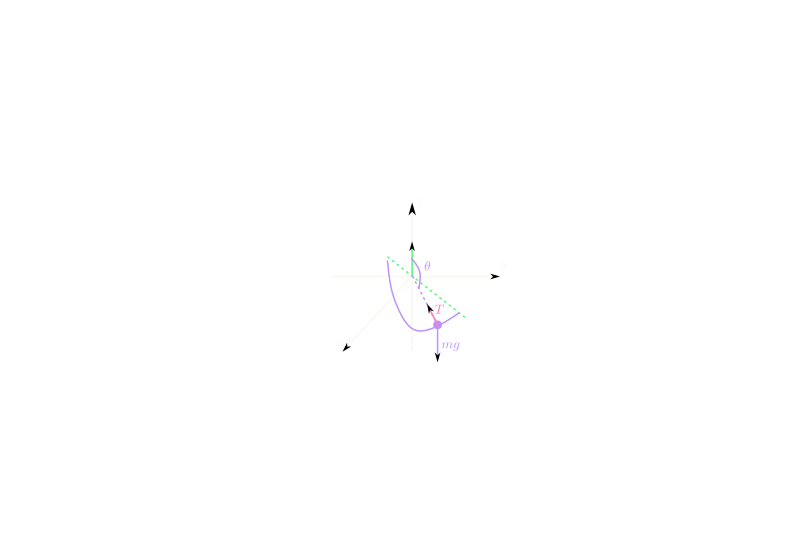
\includegraphics[width=0.5\textwidth]{hw4.png}
    \caption{Square Lattice with free electron at corner ($k_b$) and at the midpoint of a side
    face ($k_a$).}
    \label{fig:hw4_3a}
\end{figure}
The corner electron has a wave vector $\vb k_b = (\frac{\pi}{a}, \frac{\pi}{a})$ and the side face
electron has a wave vector $\vb k_a = (\frac{\pi}{a}, 0)$. The energy of the electron in the lattice 
is given by
\begin{align*}
    \epsilon = \frac{\hbar^2 k^2}{2m}
\end{align*}
so the ratio of the two electrons are
\begin{align*}
    \frac{\epsilon_b}{\epsilon_a} = \frac{k_b^2}{k_a^2}
\end{align*}
and since the square of the magnitudes of the wave vectors are
\begin{align*}
    k_b^2 = \frac{\pi^2}{a^2} + \frac{\pi^2}{a^2} = \frac{2\pi^2}{a^2} \qand k_a^2 = \frac{\pi^2}{a^2}
\end{align*}
the ratio of the energies is
\begin{align*}
    \frac{\epsilon_b}{\epsilon_a} = \frac{2\pi^2/a^2}{\pi^2/a^2} = 2
\end{align*}
(b) For three dimensions the wave vectors are
\begin{align*}
    \vb k_b =\qt(\frac{\pi}{a}, \frac{\pi}{a}, \frac{\pi}{a}) \qand \vb k_a = \qt(\frac{\pi}{a}, 0, 0) \\
    \implies k_b^2 = \frac{3\pi^2}{a^2} \qand k_a^2 = \frac{\pi^2}{a^2}
\end{align*}
so the electron at the corner has a kinetic energy larger than the electron at the side face by a 
factor of
\begin{align*}
    \frac{\epsilon_b}{\epsilon_a} = 3
\end{align*}
(c) For divalent metals—two valence electrons per atom— the fermi surface extends out of the first 
Brillouin zone and into the second. The spill over of the valence electrons and neglect filling up 
the high energy corner states causes the conductivity of divalent metals to be higher than that of monovalent metals.
\end{document} 